\chapter{Introduction}\label{chapter:introduction}

Mathematical formulae, integral to \ac{STEM} papers, often challenge readers due to the ambiguous use of variables or identifiers and their associated meanings or definitions. The constraints of the English and Greek alphabets (being finite) frequently lead to the reuse of the same identifiers with varying definitions contingent upon context. This ambiguity can be particularly daunting for those unfamiliar with the subject matter. As the visual representation in Figure \ref{fig:introduction-motivation} illustrates, disambiguating identifiers within mathematical formulae presents a considerable challenge. This challenge is particularly evident when the same variable serves multiple roles, each underpinned by a distinct definition. Such ambiguities become even more problematic for readers not profoundly acquainted with the subject matter, complicating the already demanding task of comprehending each identifier's specific meaning within the context of a complex formula.

\begin{figure}[htpb]
  \centering
  \begin{tabular}{c}
    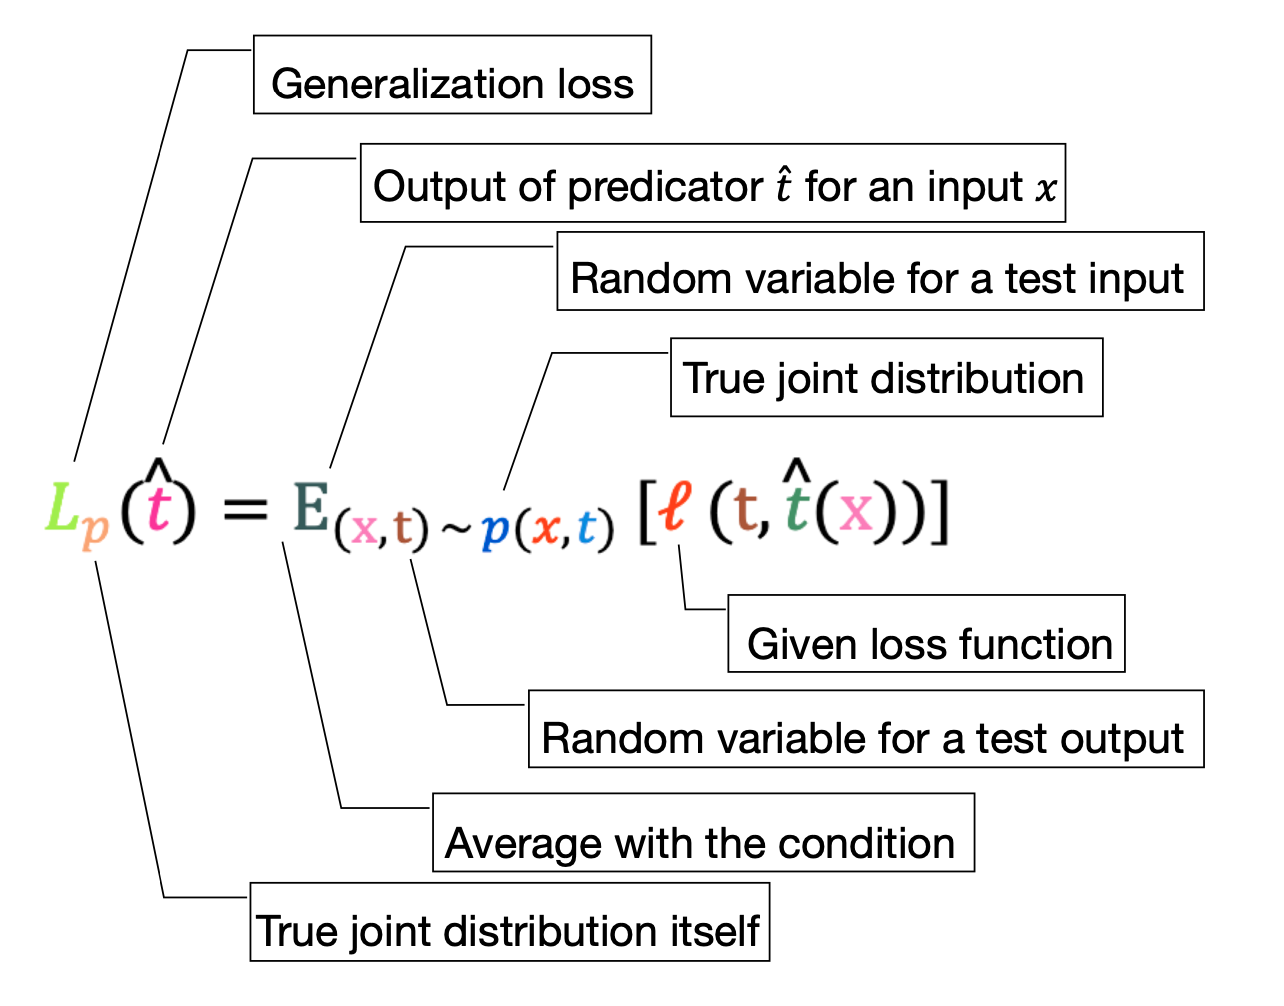
\includegraphics[width=10cm]{images/introduction-motivation.png}
  \end{tabular}
  \caption[Challenges in Disambiguation]{Challenges in the Disambiguation of Mathematical Formulae}\label{fig:introduction-motivation}
\end{figure}

%% Comments to Aamin: The arrows from "Average with the condition" and "Random variable for a test input" points "too far left, right?" (x, x, and X all still look untagged)
%% It is also unclear if "itself" makes any difference for "p" and "p"?

\href{https://github.com/wtsnjp/MioGatto/tree/main}{MioGatto} \footnote{\url{https://github.com/wtsnjp/MioGatto/}} \citep{asakura2021miogatto}, a Math Identifier-oriented Grounding Annotation Tool, was conceived to address this issue. However, manually annotating papers to define each identifier is a new challenge. This process is time-consuming and resource-intensive, often requiring a whole day for annotation, depending on the paper's length.

The concept of grounding mathematical formulae \citep{asakura2020towards} offers a promising solution. By automating this process, we can significantly expedite the annotation process. This thesis adopts a predominantly data-driven approach to develop an automation tool, which we have realised through the following stages:

\begin{enumerate}
    \item \textbf{Detecting/Retrieving:} This phase entails the transformation of the \LaTeX \space source into a machine-readable HTML/XML format using \LaTeX ML \footnote{\url{https://math.nist.gov/~BMiller/LaTeXML/}} ~\citep{ginev2011latexml}.
    
    \item \textbf{Dictionary Generation:} Leveraging \ac{LLMs}, short text clustering techniques will be employed to construct a comprehensive dictionary of all mathematical identifiers as keys with their respective possible descriptions as the corresponding values. Each paper has its dictionary.
    
    \item \textbf{Association of Each Occurrence:} This step will involve associating every instance of a mathematical identifier with its corresponding definition, drawing inspiration from MathAlign ~\citep{alexeeva2020mathalign}.
\end{enumerate}


\section{Motivation and Problem}

Annotating mathematical identifiers in scientific papers is a cornerstone for enhancing comprehension. Traditionally, this task has been performed manually, a method that, while effective, is fraught with challenges:

\begin{itemize}
    \item \textbf{Time-Consuming:} Manual annotation is inherently labour-intensive, often requiring hours or even days for a single paper.
    
    \item \textbf{Accessibility:} The expertise and resources required for manual annotation are not universally available, limiting its reach.
    
    \item \textbf{Cost Implications:} The saying "time is money" holds here. The extended hours spent on manual annotation translate to increased financial costs.
\end{itemize}

Given these constraints, there is a pressing need for a solution that's both efficient and universally accessible. Automation emerges as a promising alternative, potentially reducing annotation time from days to minutes and democratising access for a wider audience.

However, the path to automation has its challenges. Traditional \ac{NLP} techniques, such as \ac{POS} tagging or the establishment of formal grammar, tend to oversimplify the problem. These methods often provide a generalised solution, covering only a fraction of the diverse challenges presented by mathematical annotations. 

In recent years, LLMs have shown immense promise in various NLP tasks. Their capacity to "understand" and generate context-rich text suggests they could be pivotal in automating the annotation process, provided they are used effectively.

\section{Research Questions}

The primary objective of this research is to explore the feasibility and effectiveness of using LLMs to automate mathematical identifier annotations in scientific papers. To guide this investigation, we have formulated the following research questions:

\begin{enumerate}
    \item \textbf{Efficacy of LLMs:} How effective are LLMs, specifically GPT-3.5 ~\citep{openai2023} and GPT-4 ~\citep{2303.08774} and some Open Source LLMs, in generating accurate annotations for mathematical identifiers compared to traditional manual methods?
    
    \item \textbf{Contextual Understanding:} To what extent can LLMs disambiguate mathematical identifiers based on context, given the inherent polysemy of these identifiers?
    
    \item \textbf{Coverage of Annotation:} What percentage of a scientific paper can LLMs effectively annotate?
    
    \item \textbf{Accuracy concerning Ground Truth:} How closely do the annotations generated by LLMs align with the ground truth provided by manual annotations?
    
    \item \textbf{Efficiency:} How does the automation process using LLMs impact the time required for annotating scientific papers, and what are the implications for cost savings?
    
    \item \textbf{Limitations of Automation:} What are the potential pitfalls or limitations of using LLMs for this automation task?
\end{enumerate}

The answers to these questions provide a comprehensive understanding of the potential and challenges of using LLMs to automate mathematical identifier annotations.

\section{Contributions}

This research has led to several significant advancements in automated mathematical identifier annotations. The contributions of this thesis can be enumerated as follows:

\begin{enumerate}
    \item \textbf{Integration with MioGatto:} Successfully incorporated GPT-based annotation capabilities into the MioGatto platform, enhancing its potential for automated paper annotations.
    
    \item \textbf{Extensive Annotations:} Tested a range of LLMs, including GPT-3.5-turbo~\citep{openai2023}, GPT-3.5-turbo-16k, GPT-4~\citep{2303.08774}, \href{https://huggingface.co/TheBloke/Vicuna-33B-1-3-SuperHOT-8K-GPTQ}{vicuna-33b}\footnote{\url{https://huggingface.co/TheBloke/Vicuna-33B-1-3-SuperHOT-8K-GPTQ}}\citep{zheng2023judging}, and \href{https://huggingface.co/TheBloke/StableBeluga2-70B-GPTQ}{StableBeluga2}\footnote{\url{https://huggingface.co/TheBloke/StableBeluga2-70B-GPTQ}}\citep{StableBelugaModels, touvron2023llama, mukherjee2023orca}, to annotate a curated set of 40 scientific papers. This extensive annotation process serves as a comprehensive evaluation of the capabilities of these models.
    
    \item \textbf{Performance Evaluation:} Conducted a thorough evaluation and analysis of the annotation performances of GPT, \href{https://huggingface.co/TheBloke/Vicuna-33B-1-3-SuperHOT-8K-GPTQ}{vicuna-33b}, and \href{https://huggingface.co/TheBloke/StableBeluga2-70B-GPTQ}{StableBeluga2} LLMs, providing insights into their strengths and limitations.
    
    \item \textbf{Ground Truth Annotation:} Personally annotated a subset of papers to establish a ground truth, ensuring a reliable benchmark for evaluating the automated annotations.
    
    \item \textbf{CoNLL Score Approximation:} Developed a novel formula to approximate the expected CoNLL ~\citep{pradhan2012conll} score of a paper when annotated using GPT, offering a predictive tool for assessing annotation quality.
\end{enumerate}

%% Random Question from Rune: To what extent have the LLMs used in this research already been trained on the 40 papers and the existing annotation test sets for these 40 papers?

These contributions advance the field of automated annotation but also lay the groundwork for future research endeavours in this domain.

\section{Outline}

This thesis is structured to understand the challenges, methodologies, and outcomes of automating mathematical identifier annotations using Large Language Models. The subsequent chapters are organised as follows:

\begin{enumerate}
    \item \textbf{\hyperref[chapter:introduction]{Introduction:}}  This chapter sets the stage by introducing the study's motivation, research questions, and contributions, offering readers a contextual foundation for the subsequent chapters.
    
    \item \textbf{\hyperref[chapter:related_work]{Related Work:}} While the concept explored in this thesis is novel, this chapter delves into the limited existing literature that shares thematic similarities, providing a backdrop against which the current research can be compared.
    
    \item \textbf{\hyperref[chapter:methods]{Methods:}} This chapter summarises the journey of methodological exploration. It begins with initial attempts using traditional techniques like parts of speech tagging. Next, it transitions into the more successful GPT strategies, detailing the various prompts and markers employed to optimise the results.
    
    \item \textbf{\hyperref[chapter:results]{Results:}} Here, the empirical outcomes of the research are presented. The chapter summarises the scores achieved by each LLM, the methodologies used to derive these scores, and the rationale behind selecting the specific methods.
    
    \item \textbf{\hyperref[chapter:analysis]{Analysis:}} This chapter delves deep into the interpretation of the results. It provides insights into the significance of the outcomes and their correlation with other findings. It also introduces the novel formula developed during the research to estimate the CoNLL Score for a given paper. %%Which novel formula? The one for CoNNL scores?
    
    \item \textbf{\hyperref[chapter:conclusion]{Conclusion:}} This chapter focuses on synthesising the research findings, answering the questions posed at the outset and drawing conclusions on the study's implications and contributions.
    
    \item \textbf{\hyperref[chapter:future_works]{Future Works:}} The final chapter outlines potential avenues for further exploration and improvement, such as model combinations or the incorporation of emerging techniques.
    
    
\end{enumerate}

This structure provides a logical flow, guiding readers from the foundational concepts to the conclusions, and offers a holistic understanding of the research journey.

